\documentclass[a4paper, twocolumn]{article}
\usepackage{graphicx}

\title{Predicting Fuel Efficiency of Cars using Linear and Logistic Regression}
\author{M. Fjeldberg, M. Svensson}
\date{March 2026}

\begin{document}

\maketitle

\begin{abstract}
We use a dataset of 398 cars from the 1970s--80s to predict fuel efficiency. Linear regression explains 79\% of variation in MPG, and logistic regression correctly classifies 95\% of cars as fuel-efficient or not.
\end{abstract}

\section{Introduction}

In this project we try to predict how fuel-efficient a car is using machine learning. We work with the cars.csv dataset, which has information about 398 cars --- things like weight, horsepower, number of cylinders, and model year. We ask two questions: (1) can we predict a car's MPG? (2) can we classify it as fuel-efficient or not? For the first we use linear regression, and for the second logistic regression.

\section{Method}

\subsection{The Dataset}

The dataset has 398 cars with columns for MPG, cylinders, displacement, horsepower, weight, acceleration, model year, origin, car brand and model. Six cars have missing horsepower --- we drop them for linear regression and fill them with the median for logistic regression. We standardise all numeric features so they have a similar range, then split 80/20 into training and test sets.

\subsection{Linear Regression}

Linear regression learns a weight for each feature that, combined, predict MPG. We start with a basic model (OLS) and then try Ridge and Lasso regression, which add penalties to prevent overfitting. Ridge shrinks all weights a little, while Lasso can also ignore useless features entirely. We test five alpha values (0.01, 0.1, 1, 10, 100) using 5-fold cross-validation to pick the best one.

\subsection{Logistic Regression}

We create a binary label: ``efficient'' if MPG $\geq$ 23, else ``not efficient''. Logistic regression predicts a probability between 0 and 1 --- above 0.5 means efficient. We use the same numeric features plus one-hot encoded origin and car brand (turning categories like ``ford'' into numbers the model can use).

\section{Results}

\subsection{Linear Regression}

The OLS model achieves MAE = 2.42 (predictions are off by ~2.4 MPG on average), RMSE = 3.27, and R² = 0.790 (explains 79\% of variation). Ridge and Lasso did not improve results (Table~\ref{tab:linreg}), so the basic model is already a good fit.

The most important features are \textit{weight} (heavier = less efficient) and \textit{model year} (newer = more efficient). Figure~\ref{fig:actual_vs_pred} shows predictions vs actual values.

\begin{table}[h]
\centering
\small
\begin{tabular}{lccc}
\hline
\textbf{Model} & \textbf{MAE} & \textbf{RMSE} & \textbf{R²} \\
\hline
OLS & 2.42 & 3.27 & 0.790 \\
Ridge ($\alpha$=1.0) & 2.42 & 3.28 & 0.789 \\
Lasso ($\alpha$=0.1) & 2.42 & 3.30 & 0.786 \\
\hline
\end{tabular}
\caption{Linear regression model comparison.}
\label{tab:linreg}
\end{table}

Looking at the feature weights, we found that \textit{weight} has the biggest negative effect on MPG --- heavier cars use more fuel. \textit{Model year} has the biggest positive effect --- newer cars tend to be more efficient. Figure~\ref{fig:actual_vs_pred} shows how close the predictions are to the real values. Most points lie near the red dashed line, which represents a perfect prediction.

\begin{figure}[h]
\centering
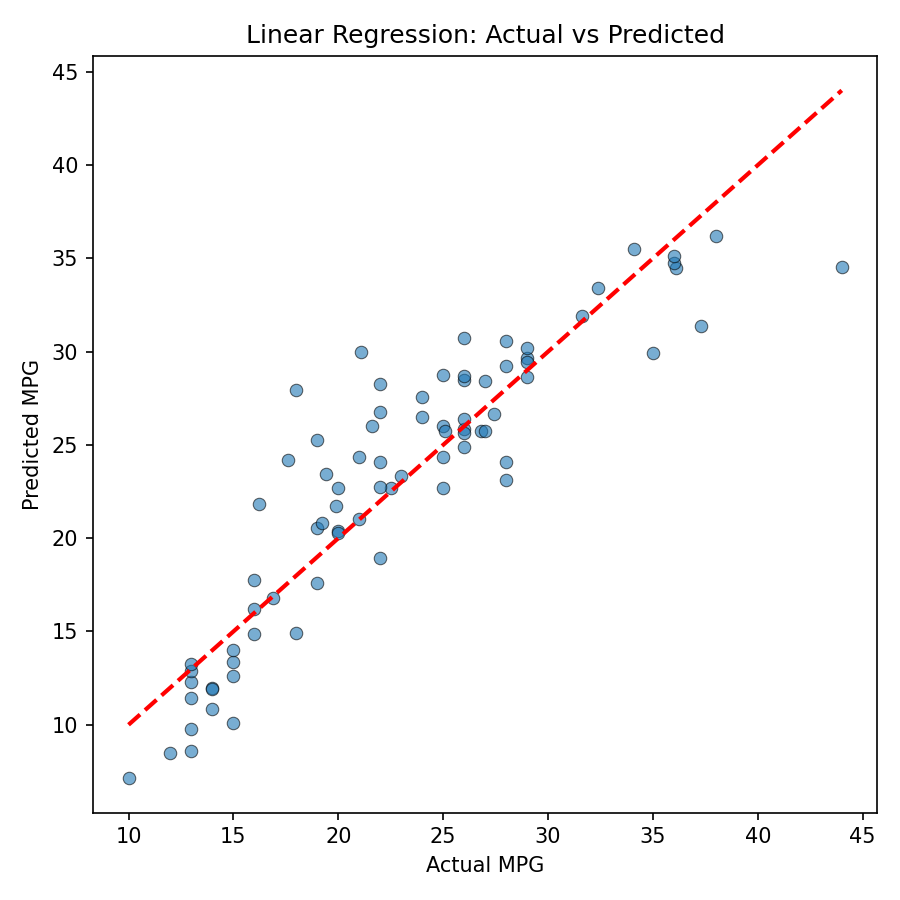
\includegraphics[width=\columnwidth]{actual_vs_predicted.png}
\caption{Actual vs predicted MPG.}
\label{fig:actual_vs_pred}
\end{figure}

\subsection{Logistic Regression}

The model correctly classifies 95\% of test cars. Only 4 out of 80 were wrong --- all cases where a non-efficient car was labelled efficient (Figure~\ref{fig:cm}). The ROC-AUC is 0.997 (Figure~\ref{fig:roc}), very close to the perfect score of 1.0.

\begin{figure}[h]
\centering
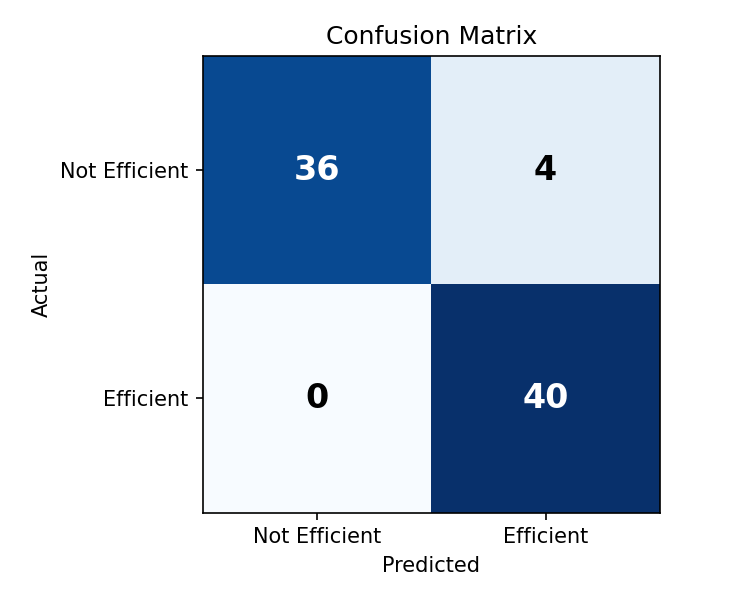
\includegraphics[width=0.75\columnwidth]{confusion_matrix.png}
\caption{Confusion matrix.}
\label{fig:cm}
\end{figure}

\begin{figure}[h]
\centering
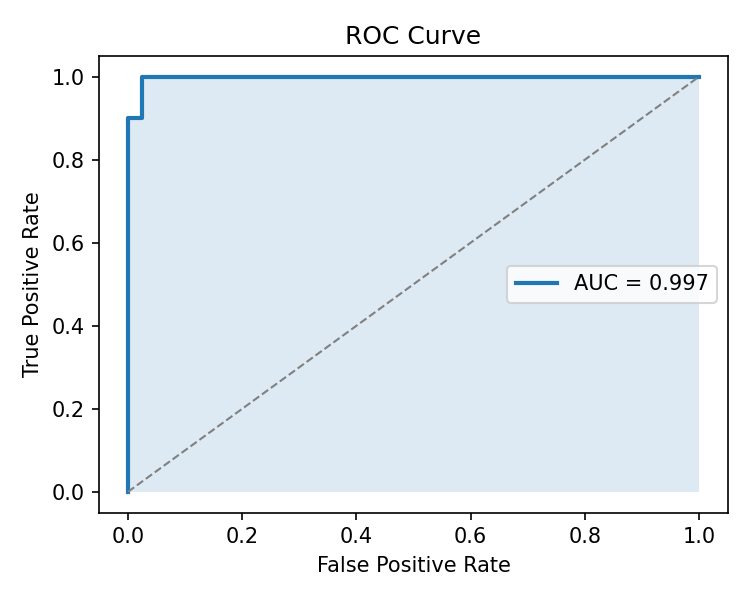
\includegraphics[width=0.75\columnwidth]{roc_curve.png}
\caption{ROC curve (AUC = 0.997).}
\label{fig:roc}
\end{figure}

\section{Conclusion}

Linear regression explains 79\% of the variation in MPG; Ridge and Lasso regularisation did not help. Logistic regression classifies cars with 95\% accuracy and near-perfect AUC. Both models show that weight and model year are the strongest predictors of fuel efficiency.

\end{document}
